\documentclass[]{article}

\usepackage{cite} % Add this line to include the cite package
% \usepackage[backref]{hyperref} % Add this line to include the hyperref package

\usepackage{amsmath} % Add this line to include the amsmath package
\usepackage{graphicx} % Add this line to include the graphicx package
\usepackage{fancyhdr}

\title{\textbf{Sys-Intro Lab1 Report}}
\author{Pan Changxun \& Liming Wang}
\date{March 2025}

\topmargin=-0.45in      %
\evensidemargin=0in     %
\oddsidemargin=0in      %
\textwidth=6.5in   
\textheight=9.0in       %
\headsep=0.25in 

\pagestyle{fancy}
\fancyhf{} % Clear all header and footer fields
\fancyhead[L]{CXP \& Sockish} % Left header
\fancyhead[C]{Sys-Intro Lab1 Report} % Center header
\fancyhead[R]{March 2025} % Right header
%\fancyfoot[L]{\leftmark} % Left footer
\fancyfoot[C]{\thepage} % Center footer
%\fancyfoot[R]{} % Right footer

\begin{document}
\maketitle

\section*{Part 1: Loop orders}
The result of the first part is shown in Figure \ref{fig:part1}.
\begin{figure}[h]
		\centering
		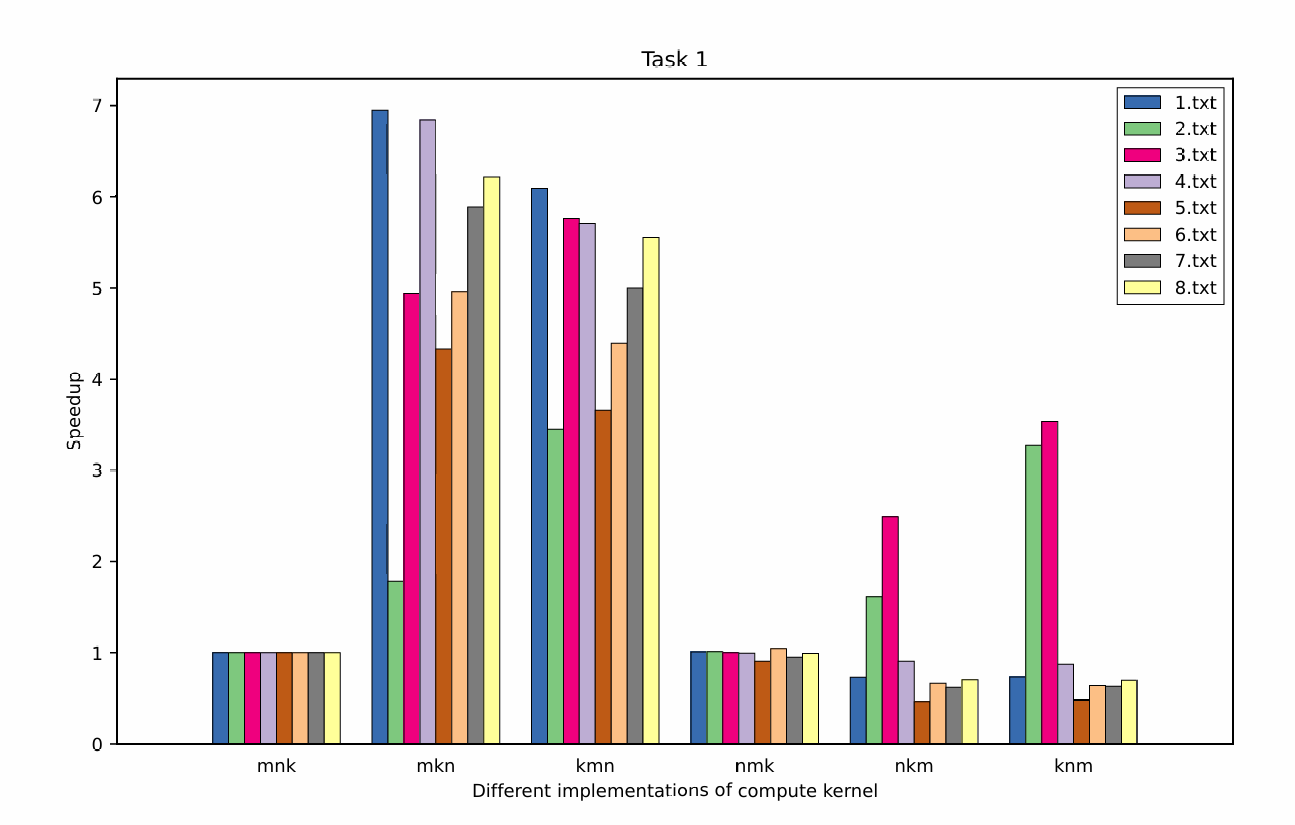
\includegraphics[width=1.0\textwidth]{task1.png}
		\caption{Part 1}
		\label{fig:part1}
\end{figure}

\newpage
\section*{Part 2: Common techniques}
The result of the second part is shown in Figure \ref{fig:part2}.
\begin{figure}[h]
		\centering
		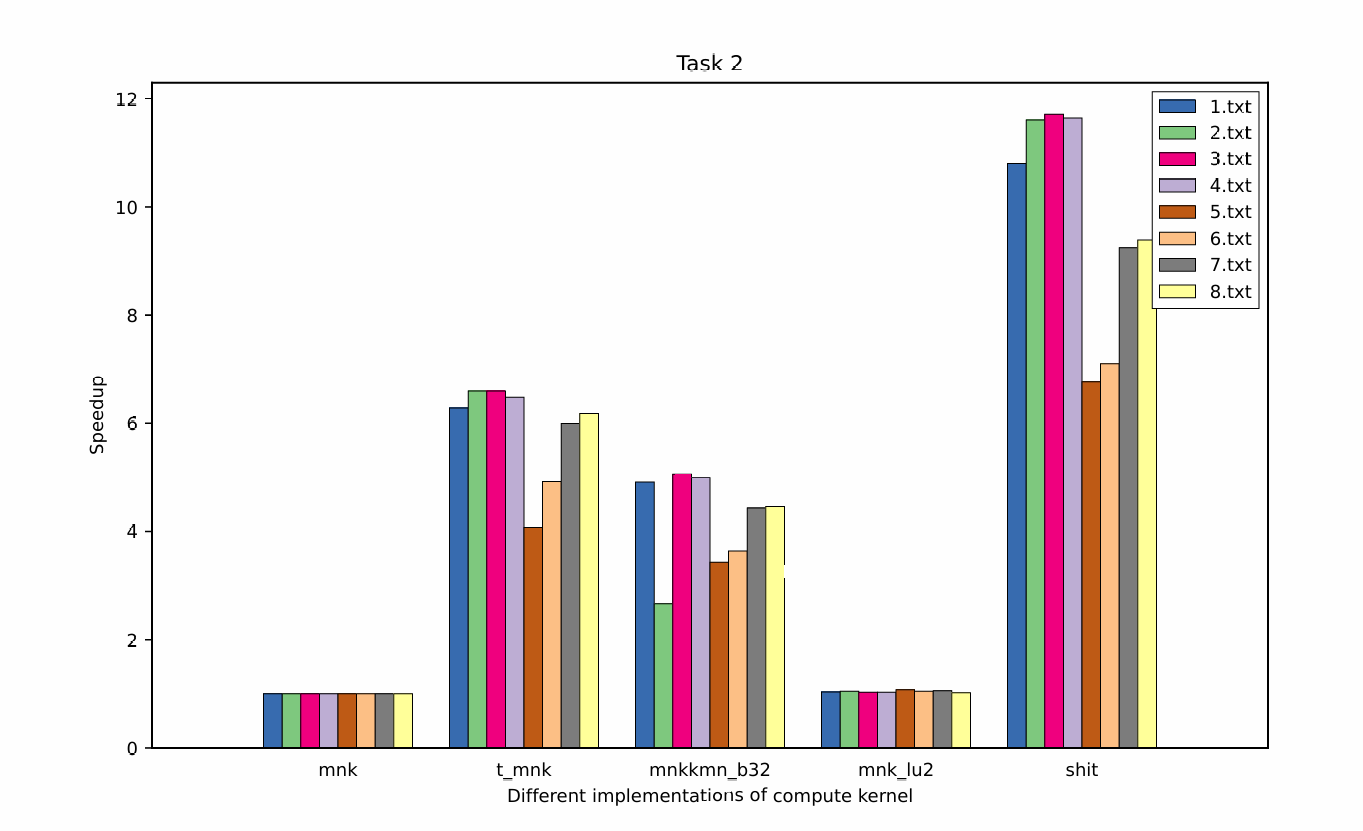
\includegraphics[width=1.0\textwidth]{task2.png}
		\caption{Part 2}
		\label{fig:part2}
\end{figure}
\\
From these, we can see that the lu2 method doesn't have a good performance to the mnk method. The t\_mnk and mnkkmn\_b32 method are better than the lu2 method. The t\_mnk method is the best one among them. Plus, we speed up the t\_mnk method by using register, it can achieve nearly 10 times faster than the original one. (which displayed in the "shit" entry)
\newpage
\section*{Part 3: With SIMD}
The result of the third part is shown in Figure \ref{fig:part3}.
\begin{figure}[h]
		\centering
		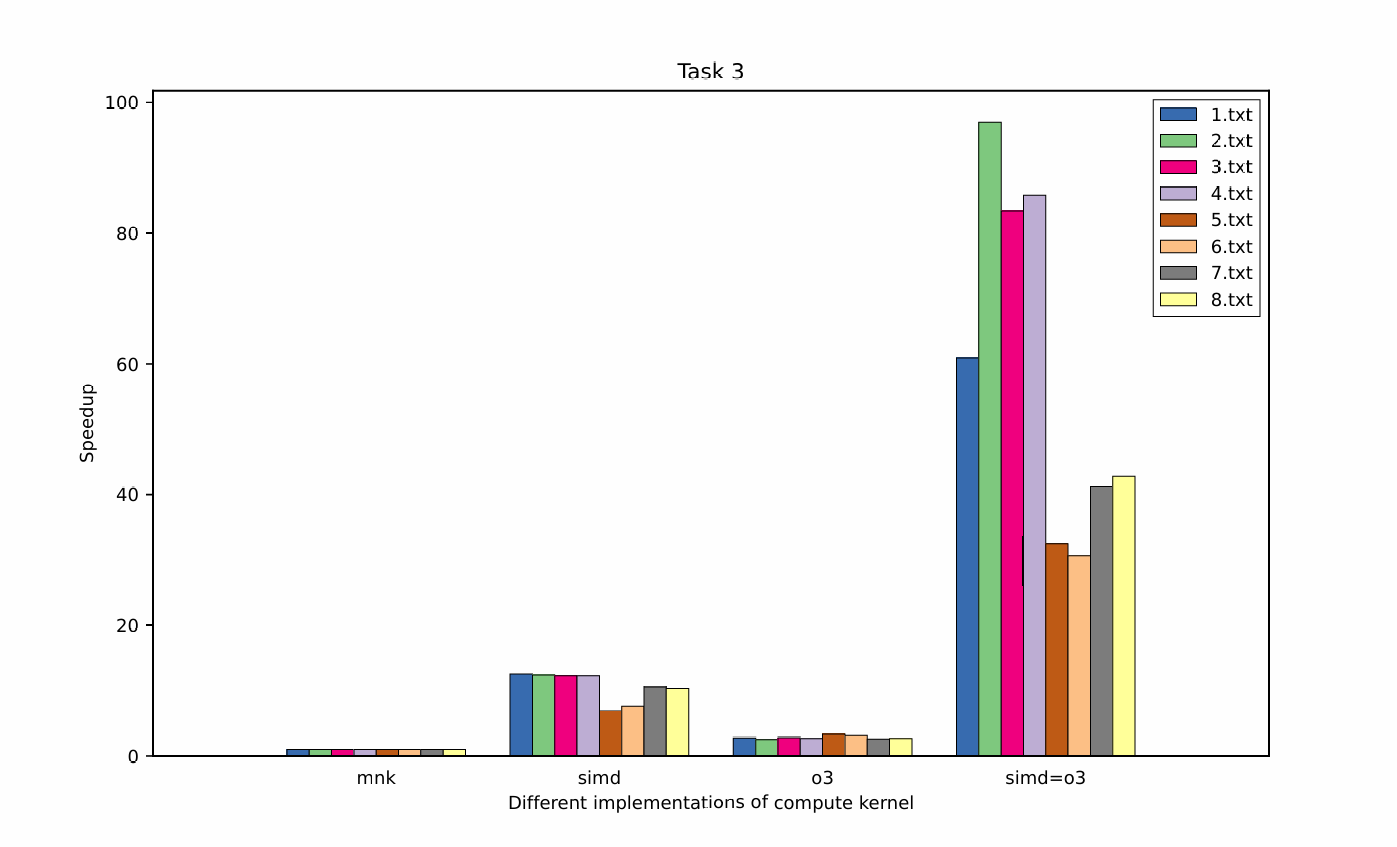
\includegraphics[width=1.0\textwidth]{task3.png}
		\caption{Part 3}
		\label{fig:part3}
\end{figure}
\\
With simd, we achieve nearly 10 times speedup. when using simd-o3, it achieves nearly 100 times than the original one.

\end{document}